\documentclass[]{final_report}
\usepackage{graphicx}
\usepackage{hyperref}
\usepackage[normalem]{ulem}
\usepackage{amsmath}
\usepackage{csvsimple}
\usepackage{float}
\usepackage[]{algorithm2e}
\usepackage[noend]{algpseudocode}
\usepackage{url}
\usepackage{listings}             % Include the listings-package
\usepackage{enumerate}


\RestyleAlgo{boxruled}
\lstset{language=Python}
\newcommand{\myparagraph}[1]{\paragraph{#1}\mbox{}\\}

%%%%%%%%%%%%%%%%%%%%%%
%%% Project details
%%%%%%%%%%%%%%%%%%%%%%
\def\studentname{Kamil Smuga}
\def\projecttitle{An approach for Continuous Capacity Planning in Cloud Environments with an Uptime-based Pricing Model}
\def\supervisorname{Prof. Liam Murphy}
\def\moderatorname{Christina Thorpe}

\begin{document}

\maketitle
\tableofcontents\pdfbookmark[0]{Table of Contents}{toc}\newpage
\listoffigures\newpage
\par{\textbf{List of tables}}

%%%%
%The most important parts of your thesis are: abstract, introduction, conclusion and
%references. These are what get read first and make that vital initial impression.
%%%
%%%
%One of first things your examiners will look at is your literature review. If they see a
%good number of journal papers, a swathe of conference papers, a few recent workshop
%papers and not too many web sites, they’ll already be impressed.
%%%
%%%%%%%%%%%%%%%%%%%%%%
%%% ABSTRACT 
%%%%%%%%%%%%%%%%%%%%%%

\begin{abstract}

\emph{ /* To be revised. */} \par
\textsl{New Infrastructure as a Service solutions are becoming available with a growing number of supported pricing models. More often than not, a hosted Cloud environment is used to design and build an infrastructure for a product. The recent availability of different pricing schemes based on resource utilization and uptime reveals new challenges in already unpredictable capacity planning process. There is a choice between ad-hoc provisioning and upfront payments with reduced hourly rates. Reserved instances charged upfront are categorized into three groups: light, medium and heavy. Which one is better for a given utilization model? When exactly does one pricing scheme becomes more cost effective? Determining which machine type is better for a given utilization model, or at which point the cost effectiveness of a pricing scheme changes, is vital for the companies subscribing to the IaaS. }

\end{abstract}
\newpage

%%%%%%%%%%%%%%%%%%%%%%
%%% INTRODUCTION 
%%%%%%%%%%%%%%%%%%%%%%

\chapter{Introduction}

\emph{ /* Type of the project: The 'Big Idea' / proof by construction. */}

\section{Description of the problem}

\section{Motivation for solving the problem}

\section{Objectives}
This work aims to design an algorithm that answer IaaS consumer's price optimality questions and help to make adjustments based on uptime based charging per machine. 

\section{Related work}

\section{Challenges}

\section{Description of methodology}
Modelling and experimentation

\section{Structure of the Thesis}
\textbf{Background}. This section will outline the background information related to IaaS consumer challenges related to understanding the whole picture for price optimality of rented infrastructure. \par
\textbf{Design}. This section explains design and environment conditions for the algorithm to be useful. \par
\textbf{Implementation}. This sections explains algorithm implementation details and data analytics software that was used - Apache Spark~\cite{spark}. \par
\textbf{Evaluation}. The proposed algorithmic approach is applied on Google Trace data~\cite{googleTrace}. \par
\textbf{Conclusion and Further Work}. The completed data analysis is discussed. Further work related to algorithm improvements, automation and lessons learned are presented. 
 
\newpage

%%%%%%%%%%%%%%%%%%%%%%
%%% BACKGROUND 
%%%%%%%%%%%%%%%%%%%%%%

\chapter{Background}

\section{The Problem Domain}
\emph{/* Description of IaaS world - providers and consumers. */}
\subsection{IaaS consumer point of view}
\subsection{IaaS provider uptime-based pricing schemes}

\section{Motivation}
\emph{ /* Description of the problem - cloud based company runs a mix of software services (real-time streaming, batch, web and database servers) on common hardware. How do they know whether provisioned VMs run in the most optimal configuration? */ }

\section{Literature review}
\emph{/* Haven't found anything that would tackle this specific problem so far. Might mention the most research is done from IaaS provider perspective? This includes resource scheduling. My work can lead to cost-aware scheduler research */}

%good number of journal papers, a swathe of conference papers, a few recent workshop
%papers and not too many web sites


%%%%%%%%%%%%%%%%%%%%%%
%%% DESIGN 
%%%%%%%%%%%%%%%%%%%%%%

\chapter{Design and Implementation}

\section{Taxonomy}

\subsection{Upfront cost}

Investment in compute resources comes with upfront cost. In case of physical machine it is hardware or lease cost. For virtual resources, IaaS providers offer per hour discounts for upfront charged schemes. \par
Upfront cost is considered to be one time payment and will be represented by \textit{u}. 

\subsection{Cost per hour}

Cost per hour represents a total cost of running a single machine divided by number of hours in calendar year. Aggregated cost is relatively easy to calculate in rented, virtualised environments. IaaS providers usually charge an X amount per hour. It might vary based on total uptime per month or pricing scheme. This number will be considered as a partial cost per hour and defined as \textit{pcph}. \par
Cost of running of physical hardware is less straightforward to calculate as it includes: power consumption, operations, hardware replacements cost, data center related costs and many others that may vary based on individual cases. Although more troublesome to calculate, cost per hour per host for physical infrastructure is possible to calculate. \par
Cost per hour will be defined as \textit{cph}. It includes upfront cost and IaaS provider per hour charges. It is defined as a function of hours of utilization per day.  

\begin{equation}
\label{eq:cph}
cph(h) = \frac{u + \sum_{i=1}^{366} pcph \times h}{365 \times h}
\end{equation}

\subsection{Intersection points between pricing schemes}

Cost per hour is calculated for each of available pricing schemes. Single result represents a matrix of hours per day and \textit{cph}. Graphical representation of results produces a graph similar to Figure~\ref{fig:cc2_8xlarge}. \par 
This representation allows to notice pricing trends. In the example below, price drops exponentially for around first 5 hours of usage and nearly stabilizes afterwards. Light is the cheapest option for around 15 hours per day usage. This is better visible on Figure~\ref{fig:cph_cc2_8xlarge_zoom}. After 15 hours, it is better to invest in Heavy utilization scheme. This is the point that will be called \textit{an intersection point} between 2 pricing schemes and noted as \textit{ip(scheme1, scheme2)}. \par
For the example below, cc2.8xlarge instance's intersection point between Light and Heavy schemes is \textit{ip(light, heavy) = 16}.

\begin{figure}[H]
	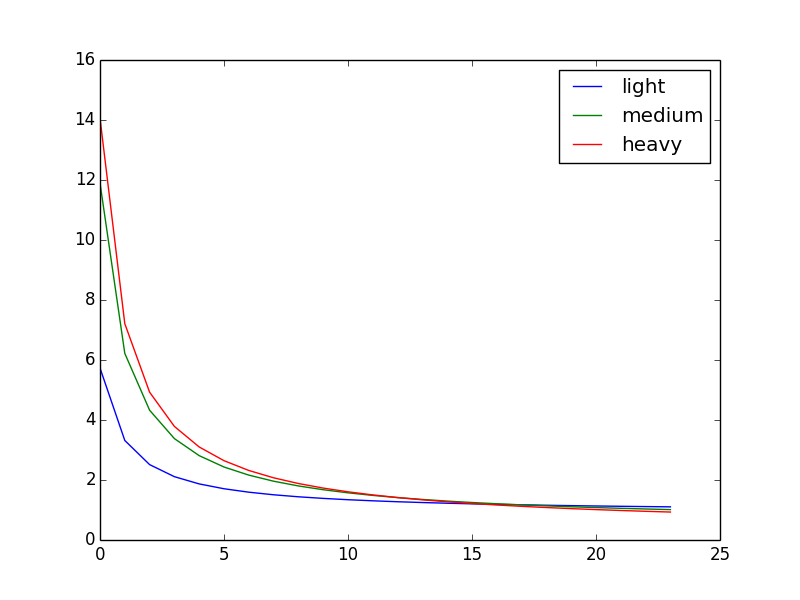
\includegraphics[width=\linewidth]{figures/cc2_8xlarge}
	\caption{\textit{cph} results for Amazon AWS cc2.8xlarge reserved instance rented for 1 year~\cite{AWS:2014}}
	\label{fig:cc2_8xlarge}
\end{figure}

\begin{figure}[H]
	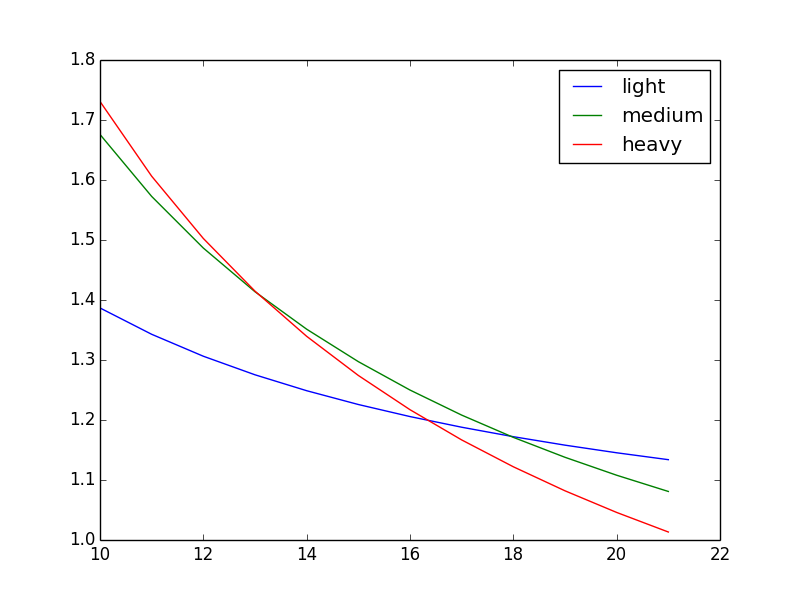
\includegraphics[width=\linewidth]{figures/cph_cc2_8xlarge_zoom}
	\caption{Zoomed \textit{cph} results for Amazon AWS cc2.8xlarge reserved instance rented for 1 year~\cite{AWS:2014}}
	\label{fig:cph_cc2_8xlarge_zoom}
\end{figure}


\section{Algorithm}

\subsection{Prerequisites} 

In order to make data-driven analysis and suggestions for optimization we need data. Below list of metrics was compiled based on algorithm needs to answer critical questions regarding state of infrastructure deployment. The list is suitable to guarantee performance SLOs only for compute nodes. Machines with significant I/O usage profile are not covered in this paper. 
Metrics can be gathered periodically, per process or per job. There are open source tools available to gather this data, e.g. collectd\footnote{\url{https://collectd.org}}, munin\footnote{\url{http://munin-monitoring.org}}, Logstash\footnote{\url{http://logstash.net}}.

\myparagraph{Machine Id}
A unique machine ID. Will be used as a key to compute further analytics.

\myparagraph{Start and End Time}
Timestamps to indicate start and end of measurement period.

\myparagraph{CPU usage}
Sampled or averaged CPU usage during measurement period. 

\myparagraph{RAM usage}
Canonical memory usage measurement. 

Metrics should be aggregated in \textless K, List\textless V\textgreater\textgreater format where K represents Machine Id and Vs are measurements. 

\subsection{Metrics data transformations and analytics}

Metrics gathered in Prerequisites section have limited knowledge about environment. Collection per job or per process produces one log line and has scope of a measurement period. Such structured data itself would not answer machine wide neither cluster wide questions. The data has to be post-processed to allow calculation of below listed aggregations and analytics.   

\myparagraph{Daily usage}

The data will be analyzed in terms of daily usage. This requires to split metrics into buckets of one day worth of data. 
It is achieved by applying a simple filter from Listing~\ref{daily_usage} in Apache Spark.

\begin{lstlisting}[label={daily_usage},caption={Daily usage filter},frame=single]

def daily_filter(line):
    day_data = line.split(",")[1]
    if (day_data == day):
        return True
    else:
        return False

for x in range(0, days_range):
    split_by_day = distFile.filter(third_filter)

\end{lstlisting} 


\myparagraph{Uptime per machine}

The aim for this metric is to find out how long a machine is up. It is a key metric that will be used to calculate optimality factors later on. Algorithm~\ref{alg:uptime_per_machine} represents pseudo code implementation and Listing~\ref{uptime_per_machine_implementation} contains implementation in Python with Apache Spark. 

\begin{algorithm}[h]
\caption{Uptime per machine}
\label{alg:uptime_per_machine}
 \KwData{Task start and end time in a form of \textless K, List\textless V\textgreater\textgreater where K is Machine ID}
 \KwResult{Number of uptime hours per machine per day}
 \algrenewcommand\algorithmicfunction{\textbf{class}}
 \algrenewcommand\algorithmicprocedure{\textbf{method}}
  \begin{algorithmic}[1]
        \Procedure{map}{$\textrm{Id } key, \textrm{List } values}$
                \State $\textsc{Emit}(\textrm{Id }key, (startTime, endTime))$
        \EndProcedure
        \Procedure{reduce for min start time}{$\textrm{Id } key, \textrm{Tuple } values}$
                \State $\textsc{Emit}(\textrm{Id }key, (a < b) ? a : b)$
        \EndProcedure
        \Procedure{reduce for max end time}{$\textrm{Id } key, \textrm{Tuple } values}$
                \State $\textsc{Emit}(\textrm{Id }key, (a > b) ? a : b)$
        \EndProcedure
  \end{algorithmic}
\end{algorithm}

\begin{minipage}{\linewidth}
\begin{lstlisting}[label={uptime_per_machine_implementation},caption={Uptime per machine implementation in Apache Spark},frame=single] 
min_start = distFile.map(lambda(line): 
                (line.split(",")[0], line.split(",")[2]))
                .reduceByKey(lambda a,b: a if a<b else b)

max_end = distFile.map(lambda(line): 
                (line.split(",")[0], line.split(",")[3]))
                .reduceByKey(lambda a,b: a if a>b else b)
\end{lstlisting}
\end{minipage}

\myparagraph{Cost per hour}

This is an implementation of \textit{cph} metric~\ref{eq:cph} defined in Taxonomy. Algorithm~\ref{alg:cost_per_hour} represents pseudo code and Listing~\ref{cost_per_hour} shows implementation in Python.

\begin{algorithm}[H]
 \caption{Cost per hour}
 \label{alg:cost_per_hour}
 \KwData{Upfront cost, Charge per hour, Uptime [hours per day];}
 \KwResult{Total cost per hour for a given pricing scheme defined as \textit{cph};}
 return (upfront + (365 * perhour * hours)) / (365 * hours)
\end{algorithm}

\begin{minipage}{\linewidth}
\begin{lstlisting}[label={cost_per_hour},caption={Uptime per machine implementation in Apache Spark},frame=single] 
def _calc_cost_per_hour(self, upfront, cost_per_hour, hours_per_day):
        return (upfront + (365 * cost_per_hour * hours_per_day)) /
                (365 * hours_per_day)
\end{lstlisting}
\end{minipage}

\myparagraph{Intersection points}

This is an implementation of \textit{ip(scheme1, scheme2)} defined in Taxonomy. This metric will be a reference point that identifies optimality points based on~\textit{cph} for various schemes. Algorithm~\ref{alg:intersection points} represents pseudo code and Listing~\ref{intersection_points} shows implementation in Python. 

\begin{algorithm}[H]
 \label{alg:intersection points}
 \KwData{Array of cph for 2 pricing schemes;}
 \KwResult{Intersection point when one pricing scheme becomes cheaper than the other one;}
 read array1\;
 read array2\;
 \ForAll{cph in array} {
 	\If{$cph2 <= $cph1} {
 		return cph
 	}
 }
\caption{Calculate intersection point between two pricing schemes}
\end{algorithm}

\begin{minipage}{\linewidth}
\begin{lstlisting}[label={intersection_points},caption={Intersection point between various pricing schemes},frame=single] 
def _calc_intersection_point(self, first, second):
   for i in range(len(first)):
      if (second[i] <= first[i]):
         return i
\end{lstlisting}
\end{minipage}

\myparagraph{Uptime Based Distance From Intersection Points}

This metric represents distance from intersection points calculated based on uptime. Result can be negative - indicates non-optimal profile - or positive otherwise. Positive and negative values can be yielded in either direction of time axis as presented on Figure~\ref{fig:distance}. 
It will be specified by flag parameter calculated together with \textit{ip(scheme1, scheme2)} results. Algorithm~\ref{alg:distance_from_optimality} represents pseudo code implementation.

\begin{figure}[H]
       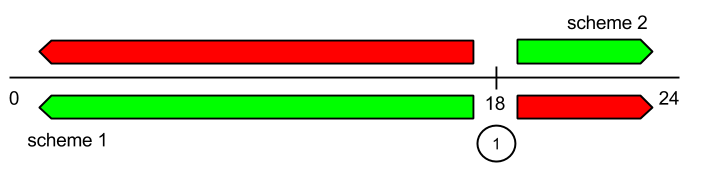
\includegraphics[width=\linewidth]{figures/distance}
      \caption{Distance from intersection points. Positive (green) values indicate optimal result. Negative (red) represent data for further improvement.}
        \label{fig:distance}
\end{figure}

\begin{algorithm}[H]
 \label{alg:distance_from_optimality}
 \KwData{Uptime, Intersection Point, Bias;}
 \KwResult{Distance from intersection point [-24, 24];}
  \If{Bias} {
        return Uptime - Intersection Point
  } 
  \Else{
        return Intersection Point - Uptime
  }
\caption{Uptime Based Distance From Intersection Points}
\end{algorithm}

Example algorithm results
\begin{enumerate}
\item Input: Uptime: 24, Optimality Point: 18, Bias: True (more optimal for values above threshold). Output: +6
\item Input: Uptime: 16, Optimality Point: 18, Bias: True (more optimal for values above threshold). Output: -2
\item Input: Uptime: 15, Optimality Point: 18, Bias: False (more optimal for values below threshold). Output: +3
\item Input: Uptime: 19, Optimality Point: 18, Bias: False (more optimal for values below threshold). Output: -1
\end{enumerate}

\subsection{Recognize inefficiencies and suggest changes}

\myparagraph{Threshold Based Report}

Generate report of machines based on distance from optimality points. Use customizable threshold. 
Results from the report will be used to calculate suggestions.

\myparagraph{Visual recognition}

Visual recognition as a helper method to define thresholds, especially for further incremental optimizations. 
Useful as static thresholds can miss a whole set of machines that are just below the threshold. 

\begin{figure}[H]
       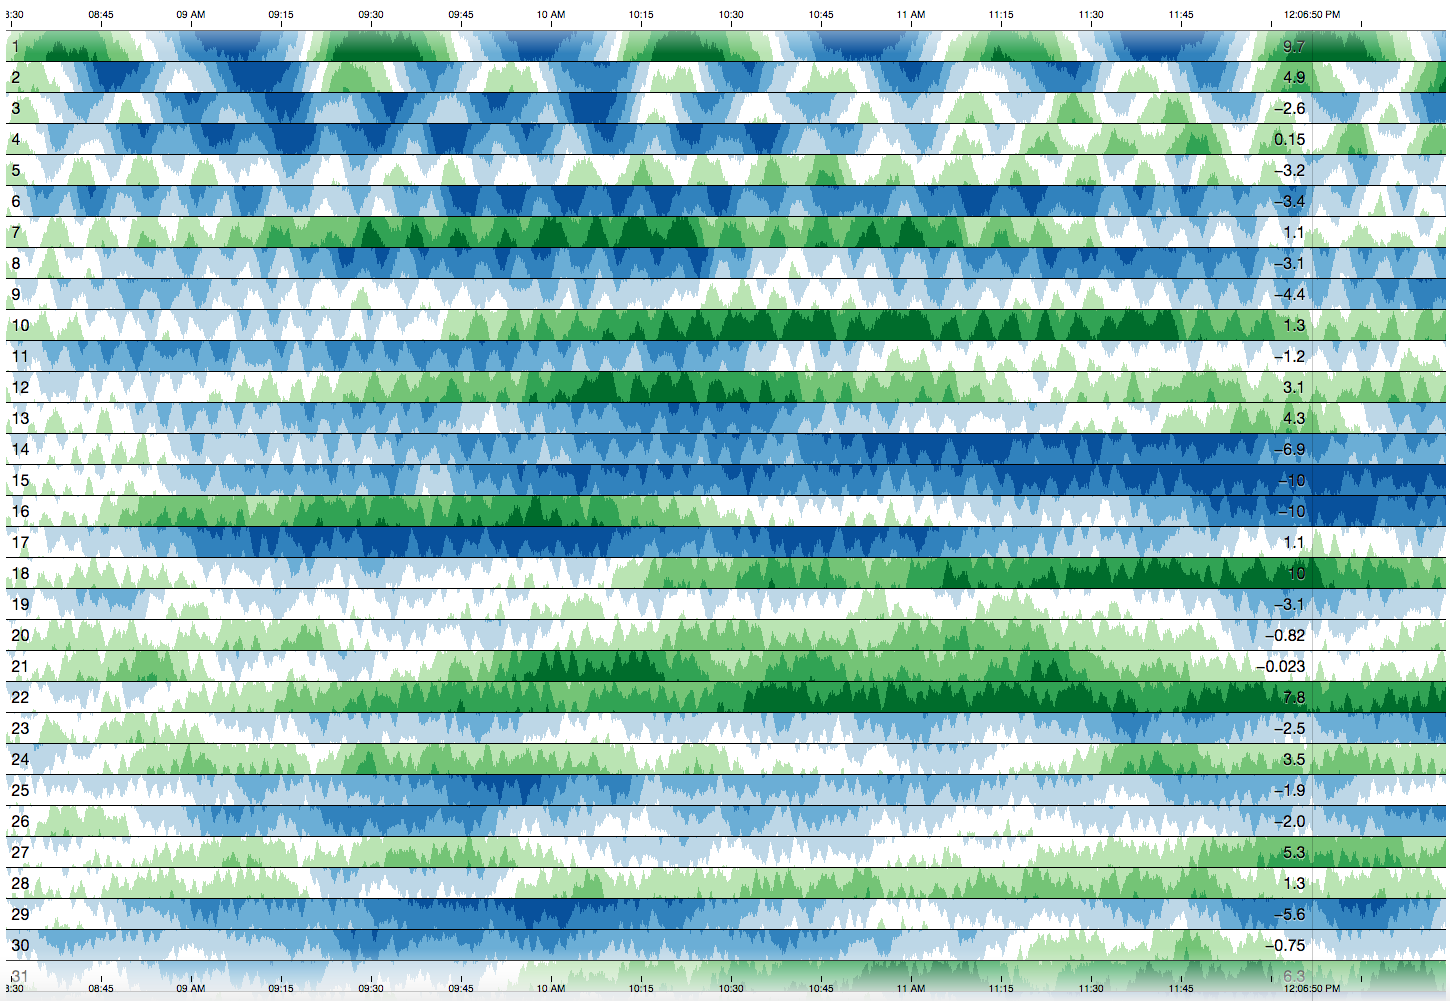
\includegraphics[width=\linewidth]{figures/cubism}
      \caption{Visualization of distance from optimality points. Green - positive, Blue - negative values.}
        \label{fig:cubism}
\end{figure}

\myparagraph{Aggregated CPU and memory usage}

Aggregated values of CPU and memory will help to suggest better utilization strategies that guarantee SLOs. Algorithm~\ref{alg:agg_cpu_mem} represents pseudo code implementation and~\ref{agg_cpu_mem_implementation} contains implementation in Python with Apache Spark.

\begin{algorithm}[h]
\caption{Aggregated CPU and memory}
\label{alg:agg_cpu_mem}
 \KwData{CPU and memory usage in a form of \textless K, List\textless V\textgreater\textgreater where K is Machine ID}
 \KwResult{Aggregated CPU and memory usage}
 \algrenewcommand\algorithmicfunction{\textbf{class}}
 \algrenewcommand\algorithmicprocedure{\textbf{method}}
  \begin{algorithmic}[1]
        \Procedure{map}{$\textrm{Id } key, \textrm{List } values}$
                \State $\textsc{Emit}(\textrm{Id }key, (cpuUsage, memoryUsage))$
        \EndProcedure
        \Procedure{reduce}{$\textrm{Id } key, \textrm{Int } aggValue}$
                \State $\textsc{Emit}(\textrm{Id }key, a + b)$
        \EndProcedure
  \end{algorithmic}
\end{algorithm}

\begin{minipage}{\linewidth}
\begin{lstlisting}[label={agg_cpu_mem_implementation},caption={Aggregated CPU and memory implementation in Apache Spark},frame=single] 
cpu = distFile.map(lambda(line): 
                (line.split(",")[0], line.split(",")[5]))
            .reduceByKey(lambda a,b: a + b)

mem = distFile.map(lambda(line): 
                (line.split(",")[0], line.split(",")[6]))
            .reduceByKey(lambda a,b: a + b)
\end{lstlisting}
\end{minipage}

\myparagraph{Calculate number of jobs per day}

Number of jobs per day will be a useful parameter to calculate cluster-wide averages used for suggestions. Algorithm~\ref{alg:jobs_per_day} represents pseudo code implementation and~\ref{jobs_per_day} contains implementation in Python with Apache Spark.

\begin{algorithm}[h]
\caption{Daily jobs count}
\label{alg:jobs_per_day}
 \KwData{Job entry in a form of \textless K, List\textless V\textgreater\textgreater where K is Machine ID}
 \KwResult{Aggregated jobs count}
 \algrenewcommand\algorithmicfunction{\textbf{class}}
 \algrenewcommand\algorithmicprocedure{\textbf{method}}
  \begin{algorithmic}[1]
        \Procedure{map}{$\textrm{Id } key, \textrm{List } values}$
                \State $\textsc{Emit}(\textrm{Id }key, 1)$
        \EndProcedure
        \Procedure{reduce}{$\textrm{Id } key, \textrm{Int } aggValue}$
                \State $\textsc{Emit}(\textrm{Id }key, a + b)$
        \EndProcedure
  \end{algorithmic}
\end{algorithm}

\begin{minipage}{\linewidth}
\begin{lstlisting}[label={jobs_per_day},caption={Aggregated CPU and memory implementation in Apache Spark},frame=single] 
def mapping(line):
    machine_id = line.split(",")[0]
    counter = 1
    return (machine_id, counter)

task_counter = distFile.map(mapping).reduceByKey(add)
\end{lstlisting}
\end{minipage}

\myparagraph{Calculate cluster averages}

Algorithm~\ref{alg:avg_cluster} represents pseudo code implementation.

\begin{algorithm}[h]
\caption{}
\label{alg:avg_cluster}
 \KwData{Daily CPU, memory usage and task count in a form of \textless K, List\textless V\textgreater\textgreater where K is Machine ID}
 \KwResult{Average CPU, memory usage and task count}
 \algrenewcommand\algorithmicfunction{\textbf{class}}
 \algrenewcommand\algorithmicprocedure{\textbf{method}}
  \begin{algorithmic}[1]
        \Procedure{map}{$\textrm{Id } key, \textrm{List } values}$
                \State $\textsc{Emit}(\textrm{Id }key, (value, 1))$
        \EndProcedure
        \Procedure{combine}{$\textrm{Id } key, \textrm{List } values}$
                \State $\textsc{Emit}(\textrm{Id }key, (currentValue + value, counter += 1))$
        \EndProcedure
        \Procedure{reduce}{$\textrm{Id } key, \textrm{Int } aggValue}$
                \State $\textsc{Emit}(\textrm{Id }key, sum / counter)$
        \EndProcedure
  \end{algorithmic}
\end{algorithm}

\begin{minipage}{\linewidth}
\begin{lstlisting}[label={avg_cluster},caption={Example code for averages in Apache Spark},frame=single] 
    sc = SparkContext(appName="avgByKey", conf=SparkConf().set("spark.driver.host", "localhost"))

    data = sc.parallelize( [(0, 2.), (0, 4.), (1, 0.), (1, 10.), (1, 20.)] )

    sumCount = data.combineByKey(lambda value: (value, 1),
                                 lambda x, value: (x[0] + value, x[1] + 1),
                                 lambda x, y: (x[0] + y[0], x[1] + y[1]))

    averageByKey = sumCount.map(lambda (label, (value_sum, count)): (label, value_sum / count))

    print averageByKey.collectAsMap()
\end{lstlisting}
\end{minipage}

\subsubsection{Squeeze-them-in suggestion strategy}

The proposed strategy calculates an amount of spare CPU and memory capacity based on cluster-wide averages. Aggregated value for CPU and memory represents an amount of capacity gathered from machines that are utilized below average. Based on the amount of aggregated capacity, algorithm will attempt to squeeze in a maximum amount of machines gathered from Threshold Based Report. As a result, it will propose to turn off a number of machines and guarantee that SLOs will be met.
This approach performs well when underutilized machines exist. For a well-balanced clusters with similar usage patterns it does not find a lot of spare capacity and would propose fairly limited improvements. 

\begin{algorithm}[h]
\caption{test}
\label{alg:squeeze-them-in}
 \KwData{Cluster averages for CPU and memory, List of machines from Threshold Based Report, List of other machines}
 \KwResult{List of machines that can be powered down}
 \algrenewcommand\algorithmicfunction{\textbf{class}}
 \algrenewcommand\algorithmicprocedure{\textbf{method}}
 %\begin{algorithmic}[1]

  %$float spare_cpu;$
  %$float spare_memory;$

 %  \ForAll{machine in Other Machines} {
%        \If{$machine.cpu \geq cluster.cpu$} {
%        \If{a}
 %              \State test % spare_cpu  cluster.cpu  machine.cpu
 %        \EndIf
%        \If{machine.memory < cluster.memory} {
%                spare_memory += cluster.memory - machine.memory
%        }
 %  }
\ForAll{machine in otherMachines}{
        \If{$machine.cpu < cluster.cpu$} {
                 $spareCpu += clusterCpu - machineCpu$
        }
        \If{$machine.memory < cluster.memory$}{
        	$spareMemory += clusterMemory - machineMemory$
        }
        %\EndIf
}
%\EndFor
% \end{algorithmic}
\end{algorithm}

Input: results of the Threshold based report. 

Computation: Calculate spare capacity based on average CPU and memory usage. Iterate through a pool of available machines (not included in input report) and advertise available capacity only if CPU and memory usage is lower than average. Aggregate spare capacity results.

Output: List of machines that can be shutdown based on computed spare-capacity.

\subsubsection{New capacity configuration suggestion}

Input: results of the Threshold based report.

Computation: Compute a minimal number of VMs for each configuration based on requested capacity

Output: A number and configuration of the cheapest computed configuration.

%%%%%%%%%%%%%%%%%%%%%%
%%% IMPLEMENTATION 
%%%%%%%%%%%%%%%%%%%%%%

\chapter{Implementation}

\emph{/* Implementation quirks related to make it work. Mostly map/reduce jobs written for Apache Spark. */}

%%%%%%%%%%%%%%%%%%%%%%  
%%% EVALUATION!!!
%%% ALGORITHM TESTING  
%%% ON GOOGLE DATASET 
%%%%%%%%%%%%%%%%%%%%%%

\chapter{Evaluation}

\emph{/* Evaluation will go through each of Design stages and will perform necessary calculations. Some examples attached below. */}

\subsection{Recognize inefficiencies and suggest changes}

\subsubsection{Threshold based report}

Generate report of machines based on distance from optimality points. Use customizable threshold. 
Results from the report will be used to calculate suggestions.

\subsubsection{Visual recognition}



\section{Methodology and setup description}

\section{Algorithm walkthrough}
\subsection{Calculate cost per hour for a given pricing scheme}
Results for ccs2.xlarge based on data published for AWS~\cite{AWS:2014} \par
\csvautotabular{out}
\subsection{Calculate intersection points to find out the best pricing scheme for a number of hours/day utilization}
%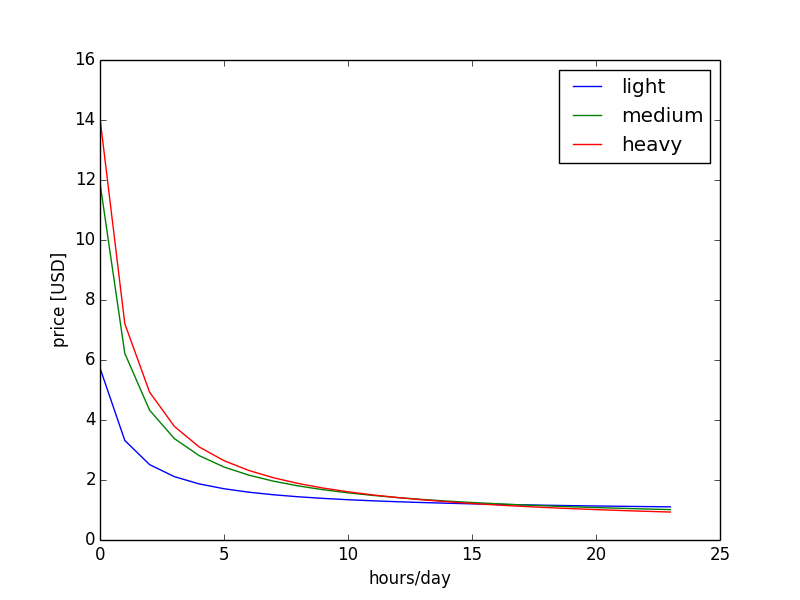
\includegraphics[width=\linewidth]{cph}
\subsection{Collect VM usage data}
\subsection{Group usage metrics by machine}
\subsection{Calculate number of hours/day, distance from optimality points, CPU and memory utilization}
\subsection{Suggest changes to the least optimal VMs considering SLAs based on CPU and memory utilization}

\section{Summary}

%%%%%%%%%%%%%%%%%%%%%%
%%% OPTIONAL!!!
%%% CAPACITY PLANNING 
%%% STRATEGIES    
%%%%%%%%%%%%%%%%%%%%%%

%\chapter{Capacity Planning Strategies}

%\section{Peak-to-mean ratio based resource assignment}

%\section{Only heavy instances}

%%%%%%%%%%%%%%%%%%%%%%
%%% CONCLUSION 
%%%%%%%%%%%%%%%%%%%%%%

\chapter{Conclusion and Future Work}

%%%%%%%%%%%%%%%%%%%%%%
%%% REFERENCES 
%%%%%%%%%%%%%%%%%%%%%%

\newpage
\begin{thebibliography}{99}
\bibitem{spark} https://spark.apache.org
\bibitem{googleTrace} https://code.google.com/p/googleclusterdata
\bibitem{AWS:2014} http://forecastcloudy.net/2012/04/02/amazon-web-services-aws-ec2-pricing-data/ https://a0.awsstatic.com/pricing/1/deprecated/ec2/ri-light-linux.json https://a0.awsstatic.com/pricing/1/deprecated/ec2/ri-medium-linux.json https://a0.awsstatic.com/pricing/1/deprecated/ec2/ri-heavy-linux.json
\end{thebibliography}
\label{endpage}

\end{document}

\end{article}